% Source: graduate-coursework/Sp26/CSCE763/Course_Assignments/Project/project_proposal.tex
% Description: Mapping of each detection method to the CSCE 763 course topics it directly exercises. {\color{USC_Garnet

\documentclass[border=4pt]{standalone}
\usepackage{amsmath}
\usepackage{amssymb}
\usepackage{graphicx}
\usepackage{tikz}
\usepackage{xcolor}
\usetikzlibrary{positioning, arrows.meta, calc, fit, backgrounds, decorations.pathreplacing}

\definecolor{USC_Garnet}{HTML}{73000A}
\definecolor{USC_Black10}{HTML}{ECECEC}
\definecolor{USC_Black70}{HTML}{5C5C5C}
\definecolor{USC_Congaree}{HTML}{1F414D}

\begin{document}
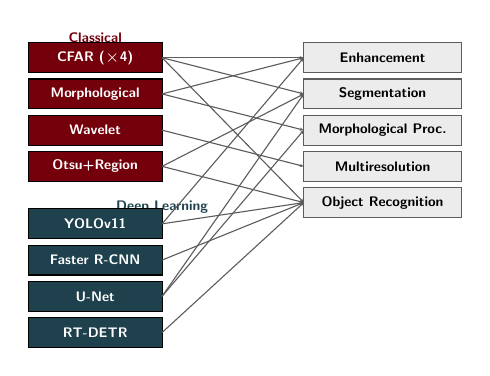
\begin{tikzpicture}[
  every node/.style={font=\sffamily\scriptsize, inner sep=2pt, outer sep=0pt},
  mnode/.style={draw, minimum height=0.38cm, minimum width=1.7cm, text=white, font=\sffamily\tiny\bfseries, anchor=west},
  cnode/.style={mnode, fill=USC_Garnet},
  dnode/.style={mnode, fill=USC_Congaree},
  tnode/.style={draw=USC_Black70, fill=USC_Black10, minimum height=0.38cm, minimum width=2.0cm, font=\sffamily\tiny\bfseries, anchor=east},
  arr/.style={-{Stealth[length=1.5pt]}, thin, USC_Black70}
]
  % Left: Methods
  \node[font=\sffamily\tiny\bfseries, USC_Garnet] at (0.85,0.25) {Classical};
  \node[cnode] (cfar) at (0,0) {CFAR ($\times$4)};
  \node[cnode, below=0.08cm of cfar] (morph) {Morphological};
  \node[cnode, below=0.08cm of morph] (wave) {Wavelet};
  \node[cnode, below=0.08cm of wave] (otsu) {Otsu+Region};

  \node[font=\sffamily\tiny\bfseries, USC_Congaree, below=0.18cm of otsu, xshift=0.85cm] {Deep Learning};
  \node[dnode, below=0.35cm of otsu] (yolo) {YOLOv11};
  \node[dnode, below=0.08cm of yolo] (frcnn) {Faster R-CNN};
  \node[dnode, below=0.08cm of frcnn] (unet) {U-Net};
  \node[dnode, below=0.08cm of unet] (rtdetr) {RT-DETR};

  % Right: Course topics
  \node[tnode] (enh) at (5.5,0) {Enhancement};
  \node[tnode, below=0.08cm of enh] (seg) {Segmentation};
  \node[tnode, below=0.08cm of seg] (morp) {Morphological Proc.};
  \node[tnode, below=0.08cm of morp] (multi) {Multiresolution};
  \node[tnode, below=0.08cm of multi] (objr) {Object Recognition};

  % Connections: Classical
  % Preprocessing (all) -> Enhancement
  \draw[arr] (cfar.east) -- (enh.west);
  \draw[arr] (morph.east) -- (enh.west);
  % CFAR -> Segmentation
  \draw[arr] (cfar.east) -- (seg.west);
  % Otsu -> Segmentation
  \draw[arr] (otsu.east) -- (seg.west);
  % Morph -> Morphological Proc
  \draw[arr] (morph.east) -- (morp.west);
  % Wavelet -> Multiresolution
  \draw[arr] (wave.east) -- (multi.west);
  % Otsu -> Object Recognition
  \draw[arr] (otsu.east) -- (objr.west);
  % CFAR -> Object Recognition (connected components)
  \draw[arr] (cfar.east) -- (objr.west);

  % Connections: Deep Learning
  \draw[arr] (yolo.east) -- (objr.west);
  \draw[arr] (frcnn.east) -- (objr.west);
  \draw[arr] (unet.east) -- (seg.west);
  \draw[arr] (rtdetr.east) -- (objr.west);
  \draw[arr] (yolo.east) -- (enh.west);
  \draw[arr] (unet.east) -- (morp.west);
\end{tikzpicture}
\end{document}
